\documentclass{scrreprt}

\usepackage{wrapfig}
\usepackage{graphicx}
\usepackage[right=3cm, top=3cm, left=3cm, bottom=3cm]{geometry}
\usepackage[T1]{fontenc}
\usepackage{lmodern}

\begin{document}

\newcommand{\HRule}{\rule{\linewidth}{0.5mm}}
\begin{titlepage}
\begin{center}

% Upper part of the page. The '~' is needed because \\
% only works if a paragraph has started.

\includegraphics[width=0.5\textwidth]{gcu.jpg}~

\includegraphics[width=0.4\textwidth]{lille1.jpg}~\\[3cm]

\LARGE Report
\HRule\\[0.5cm]
% Title
\LARGE 2D Multiplayer Video Game
\HRule\\[1.5cm]

% Author and supervisor
\begin{minipage}{0.4\textwidth}
\begin{flushleft} \large
\emph{Authors:}\\
Carl \textsc{Levasseur},\\
Pierre \textsc{Falez},\\
Benjamin \textsc{Danglot}

\end{flushleft}
\end{minipage}
\begin{minipage}{0.4\textwidth}
\begin{flushright} \large
\emph{Supervisors:} \\
Eddie \textsc{Gray},\\
Mike \textsc{Just},\\
Patrick \textsc{Lebegue}
\end{flushright}
\end{minipage}


\vfill

{\large 2012 - 2013}

\end{center}
\end{titlepage}


\chapter*{Acknowledgments} %TOREWRITE
\addcontentsline{toc}{chapter}{Acknowledgments}
First, we would like to thank Eddie Gray, our supervisor, who has supported us and
gave us lots of advice throughout this project and the Glasgow Caledonian University for
welcoming us and letting us using their comfortable facilities.\\

	  Then, we would also like to thank our French supervisor Patrick Lebegue for supporting us
	  and the University of Lille 1 for giving us the opportunity to carry out our internship in foreign country.\\

	  Finally, we wish to thank all our former professors from the University of Lille 1 who
	  permits us to achieve our graduation in very good conditions.\\

	  \chapter*{Abstract}
	  \addcontentsline{toc}{chapter}{Abstract}
	  During our 3-month-internship at Glasgow Caledonian University, we had to make a video game.
	  In this game, every player have a character, called a hero, who has characteristics, spells, and weapons.\\

	  We made it because it touched to several aspects of computer science such as database, network,
	  programming. Moreover, we had to learn a lot of stuff to get this project done.\\
		  It was also a good opportunity to work in team, and discover what advantages and disadvantages it comes with.
		  We used Git to synchronize our works, and we had a lot of issues about it, but it's part of learning.\\

		  Our project is divided in three parts. First is the client program, which is executed by any people who wants to play,
		  second is the server, and third is a shared library which contains every network functionnalities that are needed both
		  by the client and the server.\\

		  %TOREWRITE
		  To conclude this abstract we can say that this project was a great experience for many
		  reasons; we had never worked in team before, we learnt to search and develop
		  autonomy. Moreover, as it was an Erasmus placement, we could discover a new country,
		  another language, and last but not least, another culture.

		  \chapter*{Introduction} %TOREWRITE
		  \addcontentsline{toc}{chapter}{Introduction}
		  In order to validate our DUT diploma, we chose to carry out our internship in an
		  English speaking country to improve our English language.\\

		%  Our supervisor, Richard Foley, offered us a project's subject based on web and mobile
		 % technologies. We accepted it because we thought it was a really good idea to work on future
		 % technologies and it permits us to explore several fields using our computer skills acquired
		 % during our studies.\\

		  Our supervisor, Eddie Gray, let us choose our project. He gave to us the old report to saw what the other did. He let us choose technologies to do it.\\

		  The project which we choose is a Multi-player video game.??? ADD SOMETHING ???\\

		%  The project aimed to achieve a usable system by professors and able to manage
		%  multiple choice questions in an amphitheatre. Two mobile applications also had to be
		%  created so that students can answer the quiz.\\

		  This report consist of four parts. We will first expose the workplace and the project. Then, in a second part, how the application works. Finally, we will describe important technical point.
		  To conclude, we will realise an overall presentation projects results.\\
	
		%  This report consists of three parts. We will first realise an overall presentation of the
		%  project and its objectives. We will then, in a second part, describe how the system can
		%  handle the quizzes and how the corresponding mobile applications work. Finally, we will
		%  review this project and the skills acquired during these three months.

		  \renewcommand{\contentsname}{Summary}
		  \tableofcontents

		  \part{Project presentation}
		  \chapter{Workplace}
		  \section{Glasgow}%TOREWRITE
		  Glasgow is the largest city in Scotland and third most populous in the United
		  Kingdom. The city is situated on the River Clyde in the country's West Central Lowlands.
		  Today it is one of Europe's top ten financial centres and is home to many of
		  Scotland's leading businesses. Glasgow is also ranked as the 57th most liveable city in the
		  world.\\

		  In the late 19th and early 20th centuries Glasgow grew in population, eventually
		  reaching a peak of about 1 million in 1939, and was the fourth-largest city in Europe, after
		  London, Paris and Berlin. In the 1960s, comprehensive urban renewal projects resulting in
		  large-scale relocation of people to new towns and peripheral suburbs, followed by
		  successive boundary changes, have reduced the current population of the City of Glasgow
		  council area to 600,000, with 1,200,000 people living in the Greater Glasgow urban area. The
		  entire region surrounding the conurbation covers approximately 2.3 million people, 41\% of
		  Scotland's population.\\

		  The heart of the city is George Square, located in the city centre, site of many of
		  Glasgow's public statues and the elaborate Victorian Glasgow City Chambers, headquarters
		  of Glasgow City Council.\\

		  Three Universities are present in Glasgow: University of Glasgow, University of
		  Strathclyde and Glasgow Caledonian University. We achieved our project in this latter.

		  \section{Glasgow Caledonian University}%TOREWRITE
		  Glasgow Caledonian University is a public University. The university was constituted
		  by an Act of Parliament on 1 April 1993 as a result of a merger between Glasgow Polytechnic
		  and The Queen's College. It has 17,500 students from over 100 countries, almost 400
		  different courses available, a modern city-centre campus in Glasgow and high-tech facilities,
		  including the award-winning Saltire Centre library.

		  \section{Workspace}
		  The project was mainly realised in our flats because we already had everything we needed there:
		  computers, high-speed Internet connection and softwares. Moreover, we prefered to use our laptops
		  instead of university's computers because our tools were already configured.

		  \chapter{Project definition}
		  \section{Project description} %TODO Update for each functionnality implemented
		  The project consists in creating a video game where each player has its own character, also 
		  called a hero. A hero has several characteristics such as % Caracteristiques ici
		  spells, and can level up by beating his enemy. The goal depend on the game type selected by the player who created the game.\\

		  We wanted to do a multi-player video game, on network. Moreover, we want a Role Player Game where the player can truly embodies his character.\\

		  Then, we choose that project because it provide a lot of development opportunities. But of course, we couldn't do everythhing we wanted and moreover, sometimes, it was hard to know what to do in first.\\

		  In fact, at the begin we got lot of idea :
		  \begin{description}
		  \item[Multi Game Type :]{ First of all, we wanted to implements different game type in order to have a game diversify.}
		  \item[Characters Customizing :] {We wanted to give the chance to the player to have his own characters, as in physical way as in skill and spell. Thereby, each character is unique and the player can have a really role playing experience.}
		  \item[Game on network :] {We think game online are best type game.}
		  \item[Teamwork :] {We wanted to give a really importance to the teamwork. In fact, players have to collaborate with their teammates to win the game.}
		  \end{description}
		  \part{How to play}
		  \chapter{Prerequisite}
		  To be able to launch the application, you must own a MySQL database called '\emph{moba}' with following tables in it:
		  \begin{itemize}
		  \item{account (Account\_ID integer, Account\_Pseudo varchar(32), Account\_Password char(40))}
		  \item{characters (Characters\_ID integer, Characters\_Account integer, Characters\_Name varchar(32) Characters\_Level smallint(6), Characters\_Exp integer)}
		  \item{skill (Skill\_ID integer, Skill\_Characters integer)}
		  \end{itemize}

		  You can find this database in the \emph{Database} folder. You just have to import this database in your database management system with few records to get it works.\\

		  To launch the server, you just have to double click on MobaServer.exe, a console should appear showing server's logs.\\
		  It is the same for the client, double click on Moba.exe, but  you have to fill \emph{client.conf} with : "server="yourIP. If the server is on the same computer, you haven't to do that.

		  \chapter{Before the game starts}
		  \section{Login screen}
		  \begin{center}
		  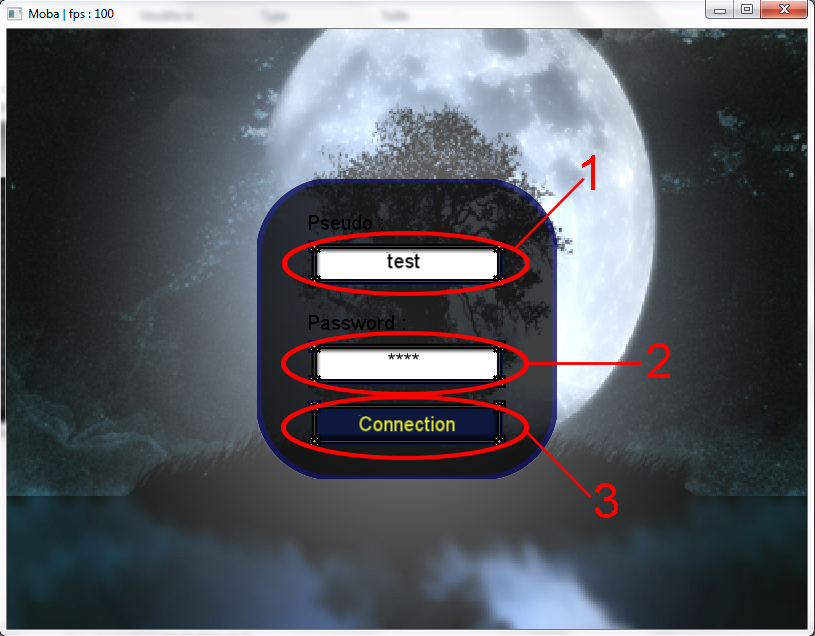
\includegraphics[scale=0.4]{connection_screen.png}
		  \end{center}
		  When you launch the client application, you're invited to connect to the server. To be able to log in, you must have a pseudo and password. Here are few login(1)/password(2) couples that are already in database:
		  \begin{itemize}
		  \item{test/test}
		  \item{test1/test}
		  \item{test2/test}
		  \end{itemize}

		  Once these fields are filled, click on connection button(3) to connect.
		  
		  \section{Managing your characters}
		  Once you're logged in, you can see the character screen.
		  \begin{center}
		  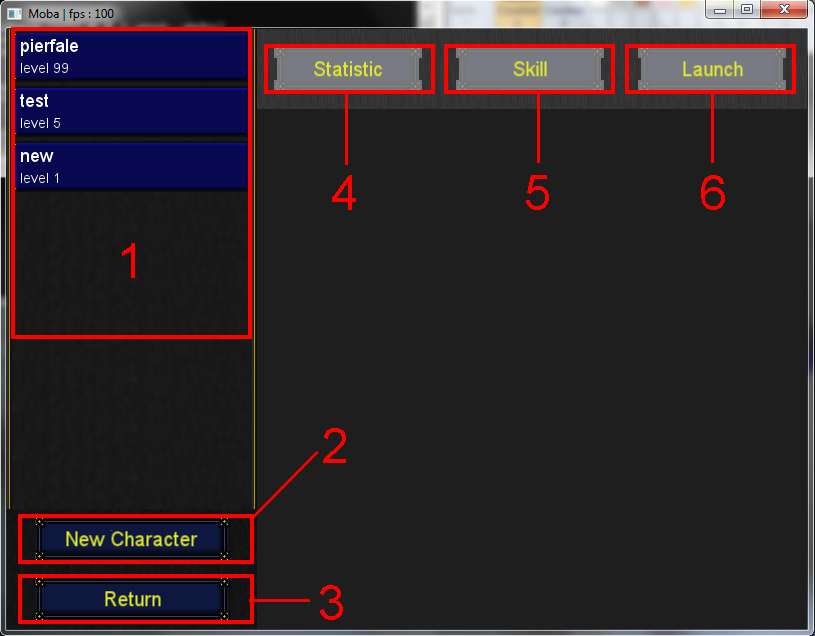
\includegraphics[scale=0.4]{character_screen.png}
		  \end{center}
		  On the left, you have your characters list(1), a 'New character' button to create a new character and 'Return' button(2) to disconnect from server. On the top, you have 3 buttons:
		  \begin{description}
		  \item[Stat(4):]{Display selected character's characteristics}
		  \item[Skill(5):]{Display the skill tree for current character}
		  \item[Launch(6):]{Go to launch screen}
		  \end{description}
		  If you don't have any character yet, you're invited to create a new one.

		  \subsection{Creating a new character}
		  \begin{center}
		  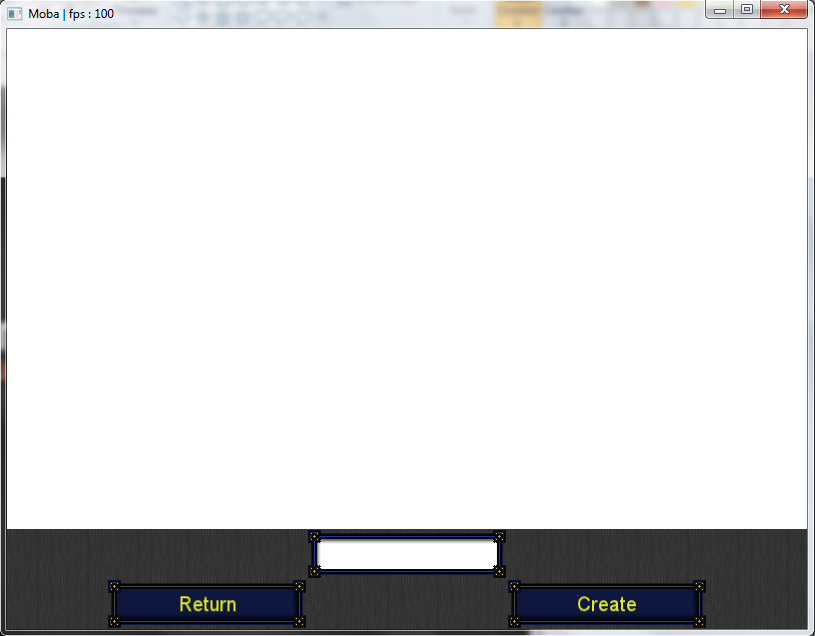
\includegraphics[scale=0.4]{create_character.png}
		  \end{center}
		  We wanted to give the opportunity to customize your character on this screen, but unfortunately, we didn't have enough time and knowledge about graphics, so we only have one skin for all characters. The textfield at bottom of the screen correspond to the name of the character.
		  \subsection{Statistics}
		  \begin{center}
		  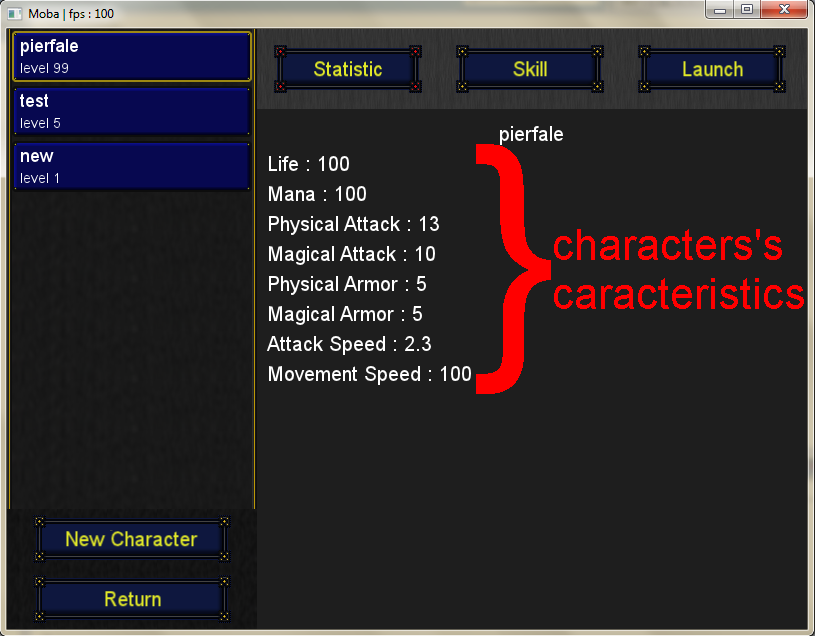
\includegraphics[scale=0.3]{stats_screen.png}
		  \end{center}
		  That screen summarize character characteristics.
		  \subsection{Skill-tree}
		  \begin{center}
		  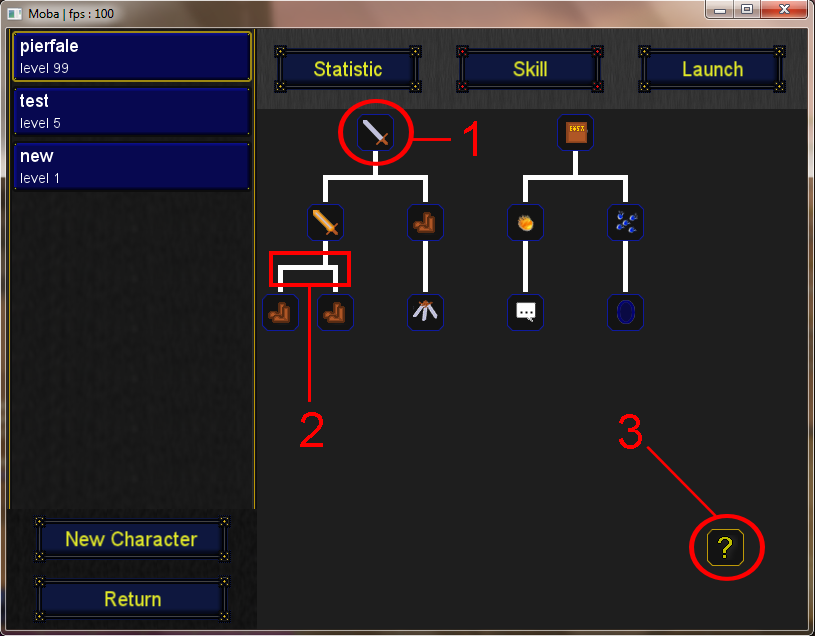
\includegraphics[scale=0.4]{skill_tree_screen.png}
		  \end{center}
		  This is the skill tree screen. Here, you can buy improvement for your character. For each level, you got one point to spend in the tree, but to get last skilsl, you must buy spells that are before and following white lines.
		  \begin{description}
		  \item[Skill(1)]{There is a skill. To buy it, you must have one point and right-click on it. If you can buy, it is appear with yellow border, if you got it with blue border but if you can't buy it, it is dark.}
		  \item[White Lines(2)]{This is the path you must follow. Example : you can not buy \emph{'PoweerFul Strike'} if you have not buy \emph{'Way of warrior'} before.}
		  \item[Help(3)]{When you put the cursor on it, a help is displayed.}
		  \end{description}
		  \section{Launch a new game}
		  \begin{center}
		  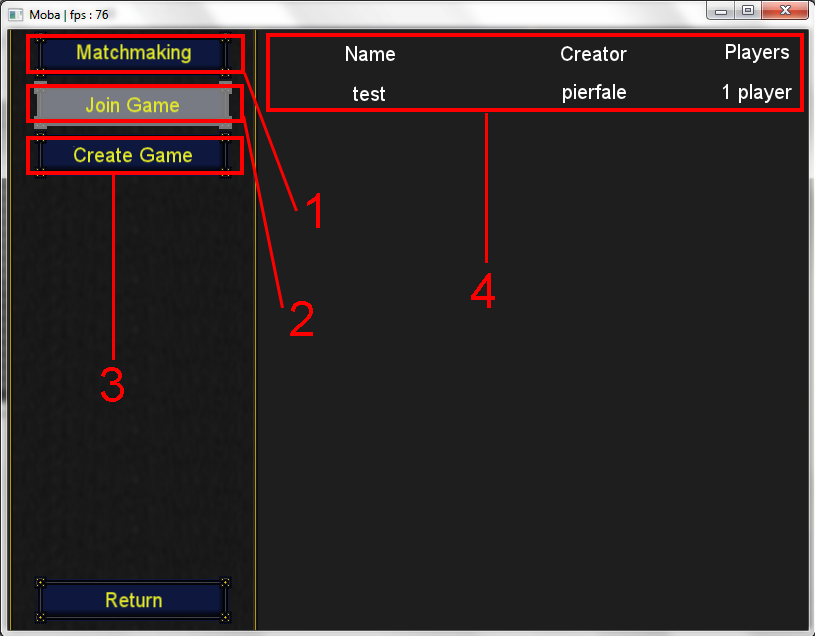
\includegraphics[scale=0.4]{launch_screen.png}
		  \end{center}
		  This screen enable you to create a new game or join an existing one. On the left, there is 3 buttons:
		  \begin{description}
		  \item[MatchMaking(1):]{Search a game where players are at the same level as you, this functionnality isn't implemented}
		  \item[Join Game(2):]{Join a game among those which are available}
		  \item[Create Game(3):]{Create a new game}
		  \end{description}
		  \section{Create a new game}
		  We wanted to give the opportunity to customize your game : game type, time, size of team... But we did not have enaugh time to implements this. The screen is similar as the screen of the creation of the characters %TODO RE-WRITE IN BETTER ENGLISH 
		  \section{Join an existing game}
		  \begin{center}
		  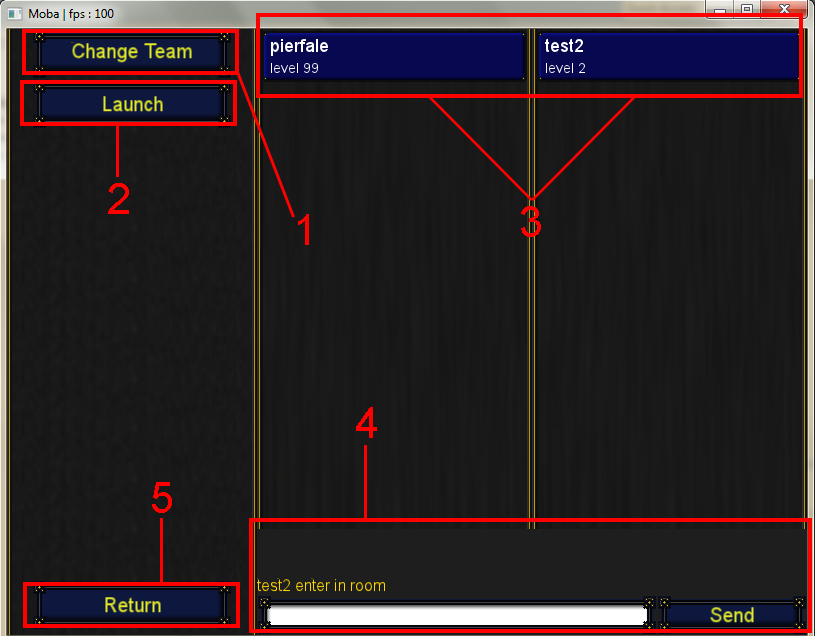
\includegraphics[scale=0.4]{lobby_screen.png}
		  \end{center}
		  This is the screen where the team are created.
		   \begin{description}
		  \item[Button Change team (1) :]{When you click on this button, your character wil change team.}
		  \item[Button Launch(2) :]{When everyone is ready to launch the game. Only the creator of the game can launch it.}
		  \item[The lobby (3) :]{We can see the both team, each players and his level.}
		  \item[Chat (4) :]{The chat to speak with other people on this game.}
		  \item[Return button (5)] {To go back at the previously screen.}
  		 \end{description}
		  \chapter{In-game}
		  \section{In-game screen}
		  \begin{center}
		  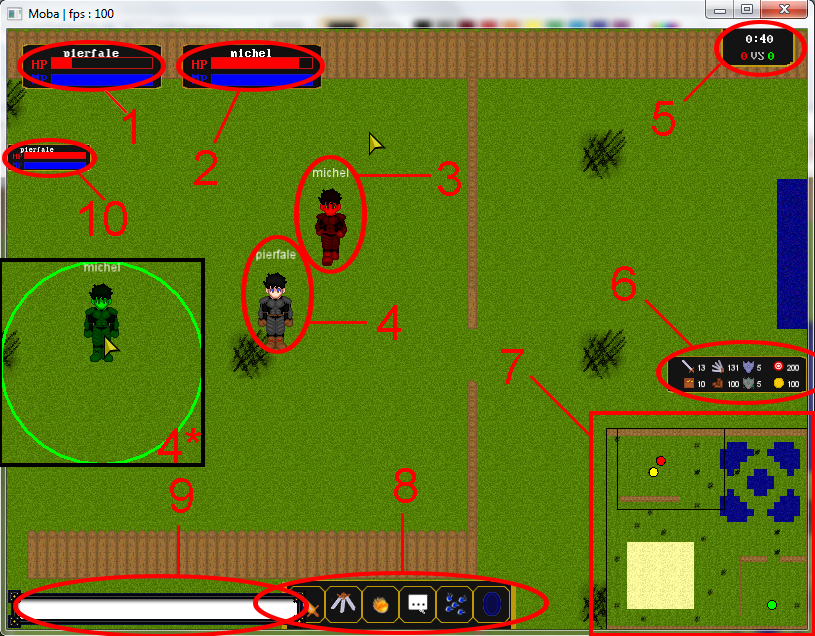
\includegraphics[scale=0.4]{in_game.png}
		  \end{center}
		  The in-game screen is composed of numerous components which display a lot of informations:
		  \begin{description}
		  \item[Character informations(1):]{The HP bar represents character's health (Health points) and the MP bar correspond to character's mana (Mana points) which are used to cast spells}
		  \item[Target informations(2):]{Same as (1) but correspond to ???targeted??? player's informations}
		  \item[Character (3) and (4):]{When the cursor is on an enemy, this one becomes red, if it's a friend, it becomes green}
		  \item[Character's range(4*):]{When your cursor is on your character, a circle representing it's maximal range for attack is drawn around him}
		  \item[Game informations(5):]{There is the time and the score}
		  \item[Character's characteristics(6):]{Contains all charactestics a player have: physical damages, magical damages, attack speed, movement speed, physical armor, magical armor, range, gold.}
		  \item[Mini map(7):]{Enable to get a global view of the entire map. Your character is represented by the yellow point, friends by green points and enemy by red points}
		  \item[Spell bar(8):]{Allow the player to cast spells, spells which are in this bar depend on your skill tree}
		  \item[Chat(9):]{A chat which permit to speak with other players}
		  \item[Friends informations(10):]{Information about all your friends in the game}
		  \end{description}

		  \section{Movement}
		To move characters, a simple left-click is required. The character will move to the location where you click.
		  \section{Attack}
		  \subsection{Auto-attack}
		To attack enemi with the auto-attack, you have to right-click on him. When you attack a enemi, he will attack you too and you will chase him.
		  \subsection{Spells}
		\begin{center}
		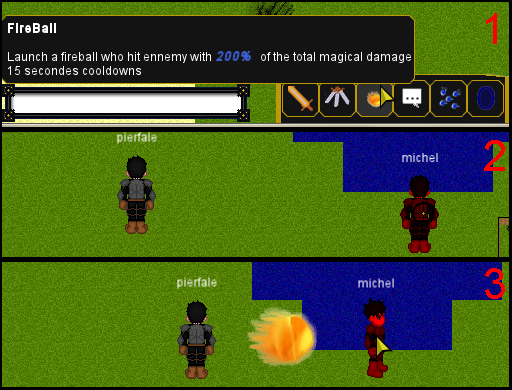
\includegraphics[scale=0.4]{cast_spell.png}
		\end{center}
		To cast a spell, you have to :
 		\begin{description}
  		\item[select a spell(1) :]{click on the spell which you want to launch by a right-click.} 
		\item[target(2) :]{Then the cursor will change and you can target your enemi.}
		\item[fire(3) :]{And with a right-click on the target, the character will cast the spell.}
		 \end{description}
		  \section{Camera}
		To move the camera, you case use arrow keys or put the cursor in the screen's border.
		  \section{How to win ?}
		There is only one game type available : DeathMatch. Two teams and one goal : have more frags than the other team before the time run out.
		  \chapter{End-game}
		  \begin{center}
		  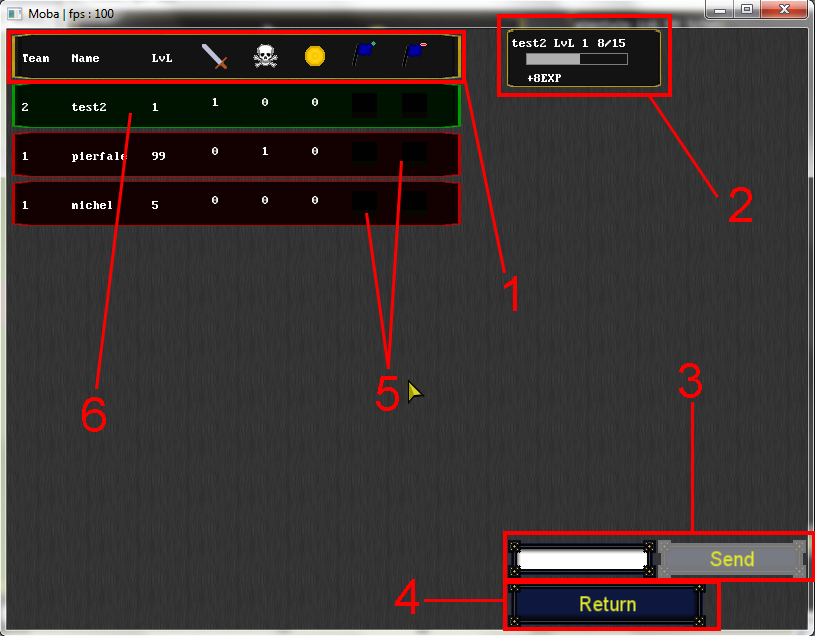
\includegraphics[scale=0.4]{end_screen.png}
		  \end{center}
		  That screen summarize the game.
		  \begin{description}
		  \item[Header(1):]It is the table's header. There is the team,  characters' name, characters'lvl, frags number, death number, gold earned, flag captured, flag get back. (gold and flag not implemented yet).
		  \item[Window experience(2):]How much experience earned, and we can see the progression.
		  \item[Chat(3):] The chat to speak with the others players.
		  \item[Return button(4):] to return to the character screen.
		  \item[enemis' window(5):] In red, we can see informations about our enemis.
		  \item[allies' window(6):] In green, we can see informations about our allies.
		  \end{description}

		  \part{Technical description}
		  \chapter{Tools}
		  \section{C++}
		  We used C++ all along this project, because it provides interesting libraries for making video games, such as SFML.
		  Moreover, JAVA is the only object-oriented language we studied at the university, so it enabled us to become multi-skilled.
		  Finally, we wanted to try the boost libraries, which allow programmers to make robust C++ programs much more easily, and improve
		  software portability.
		  \section{Eclipse CDT}
		 Eclipse is a multi-language Integrated development environment (IDE) comprising a base workspace and an extensible plug-in system for customizing the environment.\\
		We added the plug-in "CDT" : C/C++ Development Toolkit to code in C++ on Eclispe. We choose Eclispe because we used it before and it provides a very good comfort for coding. But we did not know, the plug-in does not work very well and we got some issues.
		  \section{Git}
		\begin {center}
		
\includegraphics[scale=0.5]{Git.png}
		\end{center}
		In software development, Git is a distributed version control and source code management (SCM) system with an emphasis on speed.
		We used Git to synchronyze our project faster than with others support as USB Key. In fact, for merge differents parts of the project, we spent lot of time at the begin. But now, we are able to merge a lot of source code in short time.\\
		  \section{External libraries}
		  \subsection{Boost} %TODO
		  \begin{center}
		  
\includegraphics[scale=0.75]{Boost.png}
		  \end{center}
		  Boost is a set of libraries for the C++ programming language that provide support for tasks and structures such as linear algebra, pseudorandom number generation, multithreading, image processing, regular expressions, and unit testing. Release 1.52 contains over eighty individual libraries.\\

		  Most of the Boost libraries are licensed under the Boost Software License, designed to allow Boost to be used with both free and proprietary software projects. Many of Boost's founders are on the C++ standards committee, and several Boost libraries have been accepted for incorporation into both Technical Report 1 and the C++11 standard.

		  \subsection{SFML} %TODO
		  \label{SFML}

		  \begin{center}
		  
\includegraphics[scale=0.75]{SFML2.png}
		  \end{center}

		  SFML (Simple and Fast Multimedia Library) is a portable and easy-to-use API for multimedia programming. It is written in C++ but bindings are available for C, D, Python, Ruby, OCaml, .Net. It is an object oriented alternative for the SDL.\\

		  SFML provides 2D graphics that are hardware accelerated with OpenGL. SFML can also be used for OpenGL windowing. SFML also provides different modules made to ease programming games and multimedia applications. SFML site offers complete SDK bundle in single pack, and tutorials to ease the developers. SFML Source code is provided under the terms of the zlib/png license.

		  \subsection{MySQL}
		  MySQL is the world's most widely used open source relational database management system that runs as a server providing multi-user access to a number of databases.
		  \section{Tools we developped} 
		  \subsection{Logs}
		  To make debugging easier, we made a simple log system which redirect the input stream to output stream but also into a file we ???specified???. The class used to do that is called \emph{Logs}. It contains two methods: \emph{out} and \emph{err} which ???respectively??? redirect to standard and error stream and the file described by Logs attribute. Also, using a \emph{\#define} macro, we were able to know the file's name and line were Logs methods were called, without having to send it as argument. Thus, we just had to give the message to out or err method.
		  \subsection{Configuration}
		  We also created a basic configuration tool using a parser to extract parameters values from files. Thus, we don't have to compile again each time a parameter is modified. Configuration files must match with the following format:
		  \begin{itemize}
		  \item{Key = value}
		  \item{Key = "value with blanks"}
		  \end{itemize}
		
		  Blanks between \emph{key}, \emph{'='} and \emph{value} are not ???mandatory???
		  It is also possible to put comments into these files by addind a '\emph{\#}' at the beginning of the line. The parser read each configuration files line by line and store each pair key/value in a \emph{Map} object. Finally, we developped a class to store default values if none is defined in files, so that we don't have to define a parameter if we want to keep its default value.

		  \subsection{Map editor}
		Maps are handled by a two-dimension-array which contains Case objects. Each Case object contains attributes \emph{x} and \emph{y} to describe its coordinates. Another attribute allow us to know if a character can cross it. Finally, there is an attribute which contains a texture-id so that we know how to display it. In order to get these maps persistent, we wrote it in binary files. At the beginning, we had to do it manually, but it was tedious to do, so we developped a simple program to make it easier.\\

		Both for performances and ergonomic, we decided to make a map editor, with a texture-palette. Thus, we can create new maps just by using the mouse, with two layers to handle the element overlay, then we can save it and load it into the game. The game display the map by reading its binary file, once it knows the id of each Case, it paint the corresponding texture at Case's coordinates.

		\begin{center}
		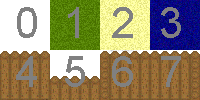
\includegraphics{image1.png}
		\end{center}
		
		\subsection{XML Parser}
		SFML has a class which permit to display text, sf::Text. But the text displayed by this class can only have a single style, single color and a single size. In order to solve this problem, we created the \emph{String} class, which inherits from \emph{Component}, and allows us to read XML files. A default style is applied to the text, but we can customize it by adding tags around ???portions de textes??? which we want to put a different style. Here are the tags availables:
		\begin{description}
		\item[<b> Text </b>]{Put the text in bold}
		\item[<br/>]{Jump to next line}
		\item[<color=r,g,b> Text </color>]{Change text's color}
		\item[<i> Text </i>]{Put the text in italic}
		\item[<size=value>Text</size>]{Change font size}
		\item[<u> Text </u>]{Underline the text}
		\end{description}

		\chapter{Graphics}
		Once we choosed to use SFML librarie (see \ref{SFML}), we had to find an additional librarie containing components to make user interfaces, because SFML only provide very basic tools, such as drawing rectangles or circles. Many people developped and distributed libraries like this, but most of them are incomplete or contain bugs, that's why we decided to make our own, based on Event-driven programming. We also choosed to make the graphic part executed by a single thread. We first tried to create thread for each component, but synchronization and concurrent access between them became to hard to manage.

		\section{???Fonctionnement Global???} %TODO
		SFML provides a \emph{sf::RenderWindow} object which contains all informations about window and enable us to draw objects which inherit from \emph{sf::Drawable}, or \emph{sf::Vertex} objects, containing vertex from OpenGL library. SFML use an event system to handle any change on the window: mouse movements, clicks, focus and so on.\\

		We created a \emph{graphics::Window} class which wrap sf::RenderWindow. Then we developped an abstract class called \emph{graphics::component} to represent a graphic component. This class contains two methods: \emph{draw} to draw a component, and \emph{event} to deal with events.
		We also created \emph{graphics::Container} class, which can contain several components. It's role is to draw all of his components. graphics::Window objects contain a graphics::Container as root component for the component-tree.\\

		While the window isn't closed, the graphics::Window object carry out each of its actions on the same thread. The order used to do these actions is important to make sure that graphic components are working correctly:
		\begin{description}
		\item[Events:]{graphics::Window get every element which are contained in SMFL event list and check if he is directly concerned by it or not\footnote{whether the window is resized or closed.}}
		\item[Listener:]{It calls all functions contained in listener-array.}
		\item[Network packets:]{process packet-list.}
		\item[Check root component:] It checks if temporary root object is different from null. If it is the case, then the old root object is recursively deleted and replaced by the new one. It happens when we want to display another screen.
		\item[Display:]{Call draw method from the root object.}
		\item[Sleep:]{If there is remaining time before next frame, then the program sleeps during this time.}
		\end{description}

		\section{Components}
		We implemented several essential components to realize this game. They all inherit from \emph{graphics::Component}. This class contains all of their common attributes:
			\begin{itemize}
			\item{Size}
			\item{Position}
			\item{State}
			\end{itemize}

			Their state can be:
			\begin{description}
			\item[normal:]{When the component has no action to do.}
			\item[hidden:]{When the user make a component hidden, it doesn't respond to events.}
			\item[disabled:]{When the user disable a component, it doesn't respond to events.}
			\item[focused:]{When the user move his mouse over the component.}
			\item[selected:]{When the user click on the component.}
			\end{description}

			The most important component is \emph{graphics::Container} which inherit from \emph{graphics::Component}. It contains several components and a layout which will ???placer??? them whenever the window is resized, or a component is either added, removed or replaced. The graphics::container object ???propage??? a lot of informations to its sons:
			\begin{itemize}
			\item{When events are received}
			\item{How to be displayed}
			\item{When the graphics::Window is modified}
			\item{When the component list is modified}
			\end{itemize}

			Each component must define its own draw and event methods.
			We also have numerous component ??????TODO????????

			\section{Layouts}
			In order to handle different sizes a window can have, we made several layouts which have to resize and move components following the size of the main window. Each graphics::Container has its own layout instance. The container is expected to destroy the old layout when it is replaced by a new one or when the container itself is destroyed. Every layout inherit from \emph{graphics::Layout} and must define the \emph{validate} method. 
			The layout knows everything about the container it belongs to, including all of its sons, so it can ???PLACER??? them correctly.
	The default layout included in a container is the VerticalLayout, which align all sons ???vertically??? and resize them ???equally???
We implemented several layouts ???for all of our needs??? (???ANNEXE???)

	\section{Events}
	At each frame, the SFML event list is ???passed??? as argument to root-container's event method. This method will send these events to all container's sons. It also contains a \emph{used} attribute which allow us to know whether an event has already been transmitted or not so that only one event is triggered when we click on two ???overlayed??? components.\\

	Each component handle its events ???differently???, some of them are ???click-insensitive???, others check if the event is sent by keyboard and so on.
	???Most components??? have an \emph{addListener} method which permit to add a new listener. These listeners ???vary??? following the component type, a button listener won't be the same as a textfield listener.\\

	When a component wants to call one of its listener's method, it gives the method and listener's reference to the graphics::Window object, which will call them ???au bon moment???

	\section{Styles}
	In order to make our components more adaptable, we decided to add classes to change component's style. Each component takes a style object as constructor argument. 
	%Pour une plus grande adaptation de nos composant nous avons décider de créer des classe pour changer leurs style. Chaque componant prend en parametre a sa construction un style. La classe de style change en fonction du component; par exemple
	%les bouton est le champs de saisie partage la meme classe graphics::BasicStyle.
	%Cette dernier (BasicStyle), est le un style qui sert areprésenter un rectangle : il prend deux parametre, le chemin vers l'image représentant les bord et le chemin vers l'image représentant le centre.
	%Cette classe découpe l'image de la facon suivante (schema?)
	%Nous avons crée une classe singleton qui charge tous les style par défault et qui permet donc de mettre facilement un style sur les component
	\section{Modeling characters}
	%Le personnage est déssiné dans 3 positions différentes (immobile, pas gauche, pas droit)pour les 4 directions possibles (SUD, EST, OUEST, NORD). Chaque direction est modélisée par un attribut int dans la classe personnage.
	The characters got three postures : motionless (repeat twice), first step and second step for four directions ( South, East, West, North). We can cut the picture in case : 
	\begin{center}
	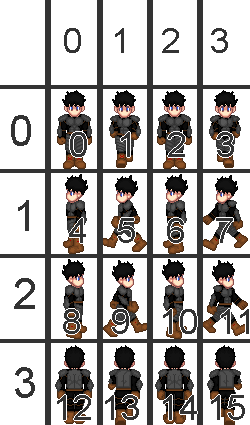
\includegraphics[scale=0.4]{char.png}
	\end{center}
	Each column is a posture, and each row is a direction. With two int in as attribute, we can manage every posture in every direction with a simple addition. For example to have the first step to the north we have :\\
		1 + 3x4 = 13, and the gameboard draw the right "case" of the character's texture.
		\section{Camera}
		The Camera object permit to display a part of map, depending on its position and its range\footnote{the window size}. Thus, the program only draw visible part of the map. We can move the camera either with the directionnal arrows or by moving the mouse on window edges. The movement is done pixel by pixel instead of case by case in order to be more fluid.

		\section{Buffer Y}
		In order to display all components, we use a buffer called \emph{Buffer Y}. At each frame, this buffer is emptied, and is filled with refreshed components (with their new positions, sizes and states). A component must inherit from \emph{graphics::BufferDrawable} to be put in the Buffer Y. This class has two methods:
			\begin{description}
			\item[getvalueY:]{Return the y-coordinate of the top left where we want to draw the component}
			\item[draw:]{Describe how the component must be drawn}
			\end{description}

			The class which manage the order in which Buffer Y's components should be drawn is \emph{graphics::BufferDraw}. It calls component's draw methods in right order so that we can apply several layers on the window.

			\section{Animations}
			All animations inherit from \emph{graphics::Animation} class which inherit from \emph{graphics::BufferDrawable}. The only attribute an animation owns is '\emph{isDone}', which is true once the animation is finished. To be displayed, an animation object calls \emph{addAnimation} method from the \emph{graphics::GameBoard} class. The gameboard's role is to add all animations which aren't finished, at each frame, to the buffer Y.\\

			Most of animations we implemented are used for spells ????TODO????\\
				%La majorité des animation que nous avons implémenter est utilisé pour les sort : la classe graphics::SingleTargetSpellAnim, qui hérite de Animation, prend en parametre le personnage qui est a l'origine du sort et celui qui est la cible.
				%cette classe possede égalment une emthode statique process qui permet d'instancier la bonne classe en fonction d'un identifiant de sort.
				%Les animation des sort sont implémenté dans graphics::SingleTargetSpellImpl.
				%Pour les animation qui sont comme un projectile, nous avons créer la classe graphics::ShotAnim qui hérite de graphics::SingleTargetSpellAnim. cette classe détermine la position de l'objet en fonction de l'angle entre le caster et la target et de la vitesse du projectile.
				%Les animation de projectile sont implémenter dans le fichier ShotImpl

				%Il y a également l'animation LifeLose qui permet d'afficher au dessus d'un personnage les point de vie que le client a retirer.

				Generally, animations are triggered after a specific packet reception. For example, mono-target spells animation are triggered when a \emph{GAME\_PLAYERLAUNCHSINGLETARGETSPELL} is received, and life loss animation when a \emph{GAME\_DOPHYSICALDAMAGE} has arrived.

				\section{Characters}
				At client side, we splitted the model and view. The model consists of two classes:
				\begin{description}
				\item[game::Character:]{Contains character's id, coordinates, direction and team}
				\item[game::Player:]{Contains character's statistics}
				\end{description}

				On the graphics part, we have:
				\begin{description}
				\item[graphics::Character:]{Inherit from graphics::BufferDrawable}
				\item[graphics::Player:]{Inherit from graphics::Character, which calculate character's position depending on its speed, previous coordinates, direction, and ???temps ecoule??? since last frame}
				\item[graphics::UserPlayer:]{Inherit from graphics::Player, represents ???WTF???}
				\end{description}

				About character's movements, we decided to let the client calculate the path to move from its position to the place where the player clicked, to avoid a server overload. However, clients' positions are always checked by the server to make sure they are not cheating.

				\chapter{Network}
				\section{libnetwork}
				%TOREWRITE MAYBE HEIN LOL
				???Since??? both the server and the client have ???network functionnalities??? in common, instead of writing these function twice, we decided to write a shared library. This library contains the network protocol.\\
					%-----------------------%

					We choosed to use TCP as transport protocol because it's more ???fiable??? than UDP. Most of datas sent over network need to be received in the right order by the ???destinataire???. To make things easier, most of network functions are executed ???synchronously???, so that we don't have to check all the time if the packet needed to allow the program to continue has arrived or not. More over asynchronous functions use several threads, which increase the program ???complexity???\\

					We defined a basic network protocol to enable clients and server to communicate. Each packet first contains the size of datas that are contained in the packet, on 4 octets, then the packet's type, which is also on 4 octets, and finally all datas. To make packet's type ???reconnaissance??? easier, we defined several types in an enumeration: the ???8 premiers??? bits are used to define the packet primary type. 3 primary types are available: \emph{Session, Game and Chat}. The 3 bits remaining are cut in differents ways depending on the packet's primary type. This system allow to deal with packets in different classes following the primary type:
					\begin{itemize}
					\item{\emph{SESSION} (0x00 XX XX XX) messages are handled by \emph{Message\_session} class.}
					\item{\emph{GAME} (0x01 XX XX XX) messages are handled by \emph{Message\_game} class.}
					\item{\emph{CHAT} (0x02 XX XX XX) messages are handled by \emph{Message\_chat} class.}
					\end{itemize}

					%Nous avons implémenter 3 type de donnée possible a envoyer : le type int (sur 4 octets), le type float (4 octets), et le type std::string. Ce dernier est envoyer de la facon suivante :
					%les 4 premier octets reorésente la longeur de la chaine et ensuite les char sont mis a la suite. Grace la a surchage des opérateur, nous avons pu redéfinir les opérateur de flux entrant et sortant
					%pour chaque type.

					\section{Server}
					The server is a console application which manage all network packets and help clients to be synchronized. Its first task during ???start up??? is to  get its configuration files and parse it. Then, it create a log file based on its configuration. Once it's done, it load all informations from the database, such as spells or skills descriptions. ???Finally???, if everything works fine, it binds a socket to the port specified in its configuration and wait for connections.
					\subsection{Access to database}
					To get all necessary datas to make the game work, the server needs an access to a database which contains these informations. That database contains accounts and characters descriptions. We made a \emph{Database} class to execute SQL queries, connect and disconnect from database. If connection to database fails, then the server closes. SQL queries which start with 'SELECT' are handled by a method which return a \emph{ResultQuery} object. This object ???encapsule??? the MYSQL\_RES structure provided by the MySQL connector and correspond to a row from querie's result. It also contains a \emph{next} method which make the ResultQuery ???pointer??? to next row and return true if it exists and false if it doesn't. ???Enfin???, it has two \emph{get} methods, the first one take an integer as argument which correspond to the column's number, and the second one take a string as argument which is the name of column we want to get the value.
					\subsection{Connection handling}
					Each client, or connection, is handled in a new thread. Whenever a new connection is opened, a new \emph{Client} object is created on server. This object handled a connection for one client. Then clients and server can communicate.

					\section{How the network protocol is used}
					\subsection{Login}
					Once the thread to handle a connection is created, it waits for a \emph{SESSION\_ASKCONNECTION} packet containing user and SHA1-encrypted password. Then, the server checks if user exists in database and if it's password is the one provided by the client. Following the result of this verification, the server reply with a \emph{SESSION\_ANSWERCONNECTION} packet and one of the following status:
					\begin{itemize}
					\item{NONEXISTENT\_ACCOUNT}
					\item{BAD\_PASSWORD}
					\item{ALREADY\_LOGGED}
					\item{LOGIN\_OK}
					\end{itemize}

					\subsection{Character selection}
					If client is ???successfuly??? logged in, it goes to character-selection screen and send a \emph{SESSION\_ASKCHARACTER} message. ???Afterwards???, the server sends a \emph{SESSION\_ANSWERCHARACTER} for each character the client owns, containing character's id, name, level and experience.\\
						Each Client object contains a \emph{Player} object as attribute. This attribute represent the character choosed by client, while the client doesn't select a character, its value is NULL. To update this value, the server must receive a \emph{SESSION\_SELECTCHARACTER} followed by the character id from the client who wants to select a character. The server make sure that the character exists and is ???associé??? to the client before changing the Player attribute's value and load all character's information from database.

						\subsection{Skills}
						When a client want to see the tree, it sends a SESSION\_ASKALLSKILLS (0x00000018) message. Then, the server reply with a SESSION\_ANSWERALLSKILLS (0x00000019) containing the number of skills the client bought and their IDs. The clients update its skill-tree afterwards, by circling in blue bought skills, in yellow for those it's allowed to buy, and in grey for those which it can't buy yet.
						When a client wants to buy a new skill, it sends a SESSION\_ASKSKILL(0x00000016) packet containing skill ID, if purchase is accepted, the server reply with a SESSION\_ANSWERSKILL (0x00000017), which also contain skill ID.\\

						For the server, each Player object contains a skill-ID-vector which represent all skills the player owns %TODO

						\subsection{Statistics}

						\subsection{Spells}
						Spells are managed in the same way as skills, they are represented by IDs, names, descriptions and icons. During a game launch, the server sends a GAME\_ALLSPELLS packet, containing all spells id and how many they are. Thus, when a client wants to use a spell, he sends a GAME\_ASKLAUNCHSINGLETARGETSPELL, if this spell is mono-target\footnote{A spell which attack only one player}, then the target ID is also included in packet. Then, the server checks several parameters such as target type, distance between players, and attack/defense bonus applied to each of them, so that it can alter spell effects correctly. Finally, it sends animation's ID to every player who are in the game.

						\part{Project results}
						\chapter{Encountered difficulties}
						\section{About the project definition}
						We choose a very good project, because it had a lot of things to do in differents aspect of computer science. But, with such a project, we got somes problems to really define what we wanted to do and with the division of labor.
						\section{About technical aspect}
						We didn't know c++ very well and using git was hard at the begin. Merging and synchronize was boring and tedious.
						\chapter{Benefits}
						\section{Programming skills}
						We improve our c++ skill,  and \\ ???SOMETHING MORE PLEASE \\
							Now, we are able to synchronize projects very quickly with git and it is really comfortable to merge with it.
							\section{Work in team}
							We learnt to listen each other, and try to solve our disagreements with compromises in order to satify each teammate.
							\section{English improvement}
							Immersion in Scotland was awesome, and our english skill was improve as we wished.
							\section{Autonomy}

							\section{Make a report}

							\chapter*{Conclusion} %TOREWRITE
							\addcontentsline{toc}{chapter}{Conclusion}
							\end{document}

							\appendix
							\chapter{}

